\section{Koncepcja i funkcjonalność aplikacji}

\subsection{Założenia przyjęte dla tworzenia aplikacji:}
    \begin{flushleft}

        \textbf{Rodzaj aplikacja:} Aplikacja internetowa (architektura klient-serwer) \\

        Aplikacja uruchamina lokalnie na komputerach oraz zdalnie na serwerze VPS. \\
        Aplikacja jest dososowana również do urządzeń moblinych. \newline\newline

        \textbf{Środkowisko lokalne:} Windows 10, Ubuntu 22.04 LTS \\
        \textbf{Środowisko produkcyjne (serwer):} VPS Linux (Ubuntu 20.04 LTS): \\ 

        \subsubsection{Środowisko uruchomieniowe:}

        \textbf{Dla Windows:}
        \begin{itemize}
            \item XAMPP 8.2.4 (serwer HTTP Apache, Serwer bazy danych MariaDB, interpreter PHP)
            \item PHP 8.2.4 Development Server
        \end{itemize}
            
        \textbf{Dla Ubuntu:}
        \begin{itemize}
            \item PHP 8.1.2-1ubuntu2.14 Development Server (serwer HTTP + interpreter PHP)
            \item Docker : obraz MySQL server version: 8.2.0 + phpMyAdmin
            % \item mysql-server  ver 8.0.34-0ubuntu0.22.04.1 (serwer bazy danych MySQL)
        \end{itemize}

        \textbf{Dla VPS:}
        \begin{itemize}
            \item Serwer HTTP Apache2
            \item Serwer MySQL
            \item Interpreter PHP 8+
        \end{itemize}
        
    \end{flushleft}

\pagebreak


\subsubsection{Cechy}
\begin{enumerate}
    \item Zastosowanie statycznego typowania (zmiennych, funkcji, metod, pól klasy), podobnie jak w językach C/C++, Java, C\#. Jest to bardziej przewidywalene i pozwala narzucić określony typ np. zwracanej zmiennej, aby uniknąć wielu błędów. Domyślnie PHP nie wymaga statycznego typowania.
    \item Podział projektu na wiele plików według struktury MVC Model-View-Controller (pol. Model-Widok-Kontroler):
        \begin{itemize}
            \item Model jest pewną reprezentacją problemu bądź logiki aplikacji.
            \item Widok opisuje, jak wyświetlić pewną część modelu w ramach interfejsu użytkownika. 
            \item Kontroler przyjmuje dane wejściowe od użytkownika i reaguje na jego poczynania
        \end{itemize}
    \item Logika aplikacji będzie zawarta w sposób obiektowy w klasach, każda klasa to osobny  plik.
\end{enumerate}

\subsubsection{Ograniczenia:}
    \begin{itemize}
        \item PHP jest podatny na pewne rodzaje ataków, takich jak na przykład wstrzykiwanie SQL, dlatego bezpieczństwo aplikacji nie jest na najwyższym możliwym poziomie i szczegłówa konfiguracja zabezpieczeń nie jest łatwa do wdrożenia w krótkim czasie
        \item PHP jest językiem interpretowanym dlatego wydajność w stosunku do języków komplilowanych jest niższa
        \item PHP nie posiada wszystkich elementów obiektowowych znanych z innych języków
        \item Ograniczony czas, przez co nie można zawrzeć wszystkich celów w wzorcowy sposób zgodny w 100\% z dokumentacją
        \item Ograniczenie aktualnej wiedzy, przez co niektóre elementy projektu mogą stanowić wyzwanie
        \item W naszej aplikacji proces logowania ogranicza się do jednego super użytkownika, którego poświadczenia są statycznie zapisne w pliku \textbf{KonfiguracjaApp.php} jako tzw. \textbf{plain text} (niezahaszowane hasła przechowywane jako zwykły, łatwy do odczytania i przechwycenia tekst), jest to zła praktyka jednak chcieliśmy uprościć tę część aplikacji ponieważ oddalała się ona dość znacząco od pierwotnego tematu, a wymagała dość dużo nadprogramowej pracy.\\
        Plik konfiguracyjny \textbf{KonfiguracjaApp.php}:
        \lstinputlisting{./src/code_snippets/oop-php/KonfiguracjaApp.php} 
        
    \end{itemize}

\pagebreak

\subsection{Narzędzia programistyczne:}
    \begin{flushleft}
        Język: \textbf{PHP 8+ OOP} \\
        Dodatkowe biblioteki: \textbf{mysqli} (łączenie się z bazą danych)\\
        Dodatkowe technologie: \textbf{HTML,CSS, JavaScript, MySQL, FontAwesome}(ikonki) \newline\newline

        \textbf{Visual Studio Code + PHP Code Extenions}: IDE (Zintegrowane środowisko programistyczne)\\
        \textbf{JetBrains PhpStorm}: IDE (Zintegrowane środowisko programistyczne)\\
        \textbf{XAMPP}: środowisko uruchomieniowe dla Windows \\
        \textbf{Docker}: konteneryzacja bazy danych lokalnie\\
        \textbf{GIT} – System Kontroli Wersji\\
        \textbf{phpMyAdmin} - graficzna nakładka na serwer MySQL, ułatwiająca operacje na bazie danych\\
        \textbf{Brave, Google Chorme}– przeglądarka internetowa posiadająca narzędzia Chrome DevTools \\
        \textbf{Microsoft Egde}– przeglądarka internetowa oraz rozbudowany czytnik plików PDF \\
        Pakiet \textbf{make} – automatyzacja poleceń w terminalu\\
        \textbf{FileZilla} – klient FTP\\
        \textbf{LaTeX} - skład tekstu do sprawozdania\\
        \textbf{PlantUML} - narzędzie do tworzenia rysunków i schematów, z poziomu pików tekstowych\\
        \textbf{Trello} – zarządzanie zadaniami w zespole\\
        \textbf{Figma} – Prototypowanie wyglądu aplikacji \\
        \textbf{GIMP 2.10.34} – Prosta edycja oraz tworzenie grafiki rastrowej \\


    \end{flushleft}
\pagebreak

\subsection{Wykaz funkcjonalności aplikacji}
    \begin{flushleft}
        Interfejs webowy, zarządzanie bazą danych z poziomu przeglądarki internetowej:

        \begin{itemize}
            \item edycje, usuwanie, dodawanie nowego piłkarza,
            \item sortowanie oraz wyświetalnie zdjęć,
            \item wyszukiwanie po nazwisku, imieniu itp.
            \item filtrowanie szczegłówe po np. kraju, pozycji itp.
            \item logowanie oraz autoryzacja użytkownika przeglądającego aplikacje
            \item dodawanie/edycje, zdjęcia piłkarza\newline\newline
        \end{itemize}


         Użytkownik może za pomocą przegląrki internetowej:
        \begin{itemize}
            \item  połączyć się z serwerem na którym hostowana jest aplikacja
            \item zalogować się do panelu poprzez formularz logowania, uzyskać autoryzacje
            \item Panel umożliwia przeglądanie katalogu  piłkarzy w przystępnej formie oraz inne operacje (edycja, usuwaniem, filtrowanie itp.).
            \item Użytkownik końcowy (klient) nie musi posiadać znajomości obsługi relacyjnej bazy danych aby w intuakcyjny sposób zarządzać aplikacją.
        \end{itemize}


    \end{flushleft}
    \pagebreak

\subsection{Prototyp}
    Prototyp graficzny interfejsu użytkownika. Wykonane w programie Figma.
    \begin{flushleft}
        \begin{figure}[!htb]
            \centering
            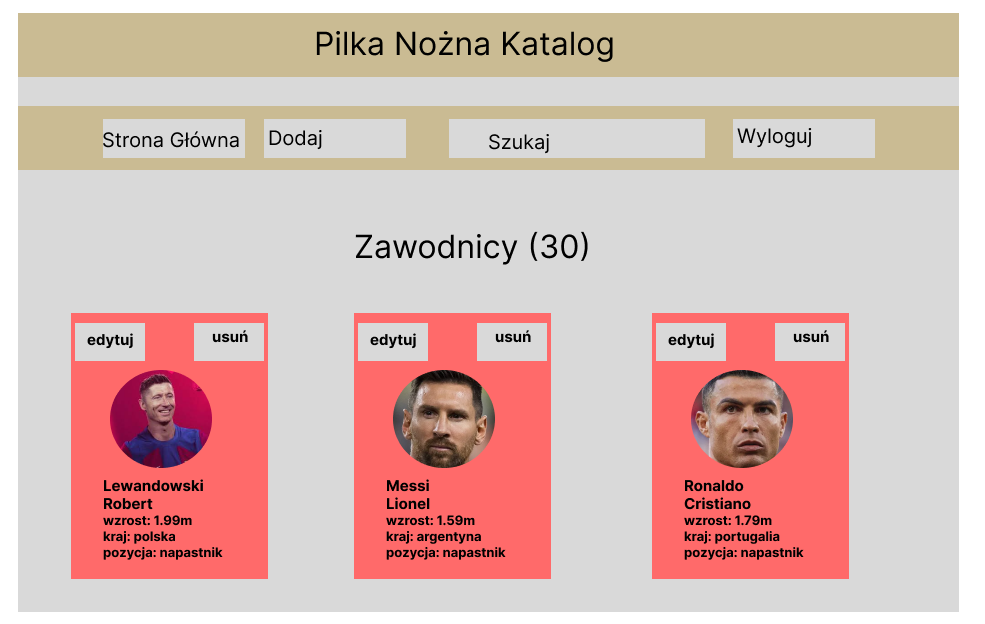
\includegraphics[width=0.5\textwidth]{1-prototyp}
            \caption{Widok strony głównej}
        \end{figure}

        \begin{figure}[!htb]
            \centering
            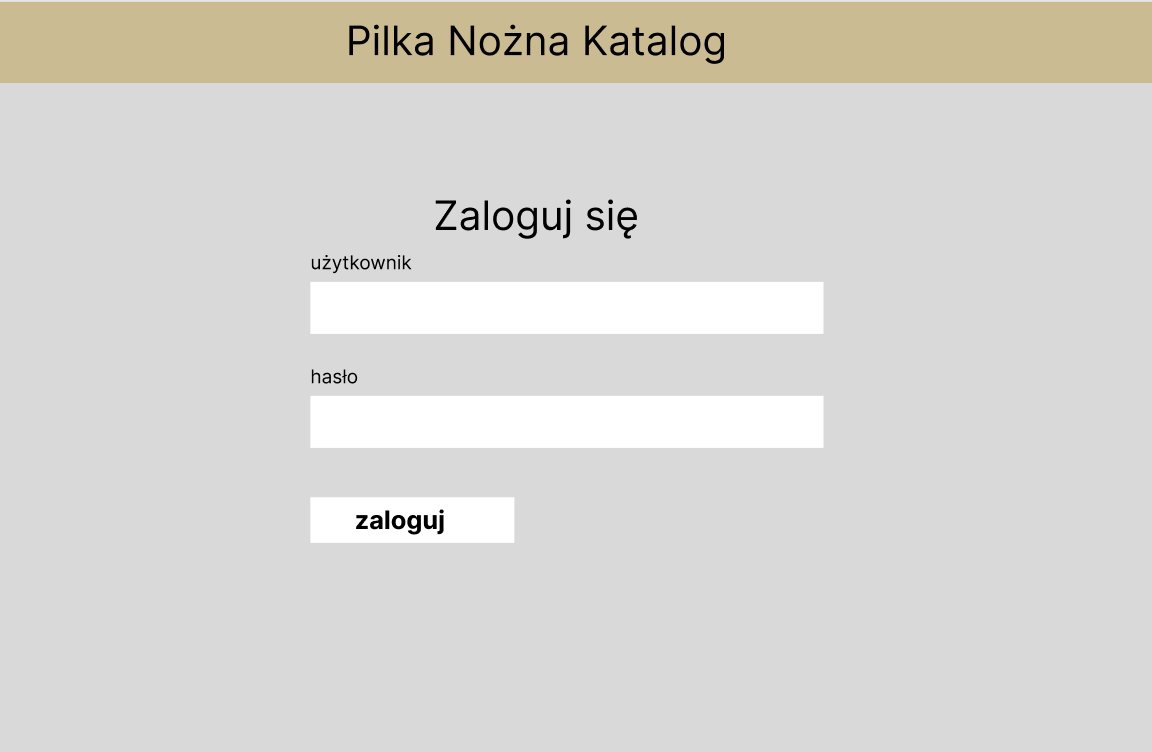
\includegraphics[width=0.5\textwidth]{2-prototyp}
            \caption{Widok ekranu logowania}
        \end{figure}

        \begin{figure}[!htb]
            \centering
            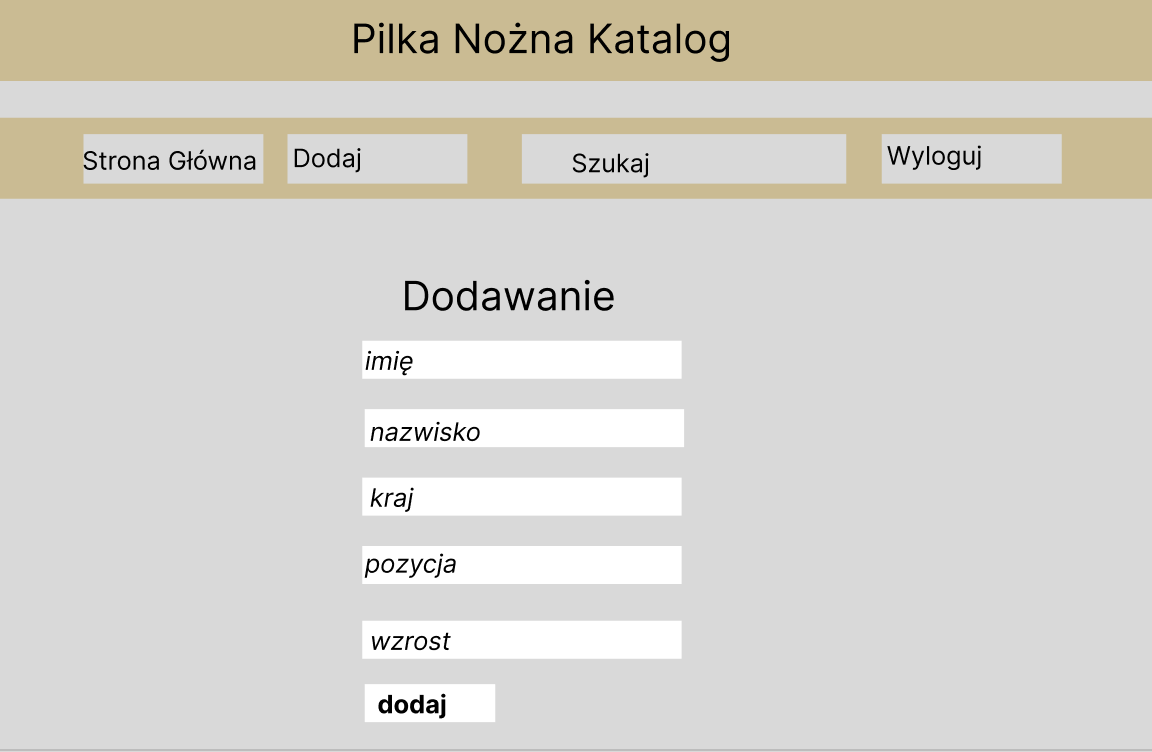
\includegraphics[width=0.5\textwidth]{3-prototyp}
            \caption{Widok strony głównej}
        \end{figure}

        \begin{figure}[!htb]
            \centering
            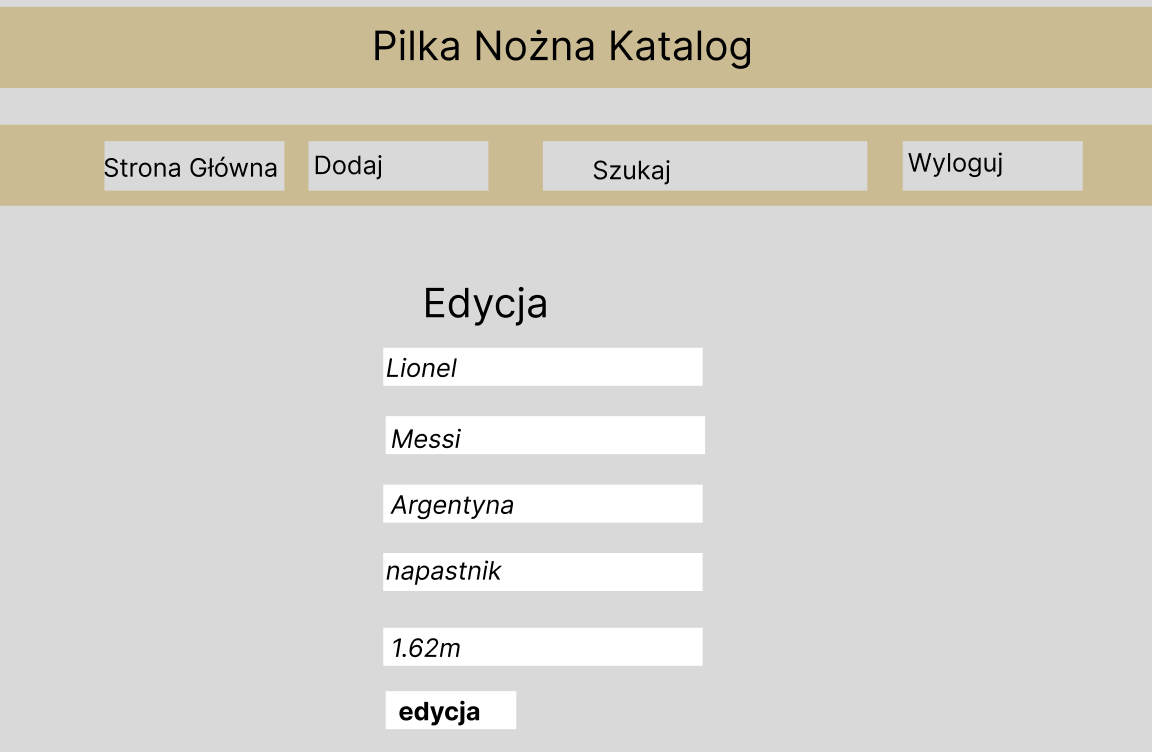
\includegraphics[width=0.5\textwidth]{4-prototyp}
            \caption{Widok strony głównej}
        \end{figure}   
    \end{flushleft}
